\documentclass[a4paper]{article}

\usepackage[english]{babel}
\usepackage[utf8]{inputenc}
\usepackage{amsmath}
\usepackage{graphicx}
\usepackage[colorinlistoftodos]{todonotes}
\usepackage{pdfpages}
\usepackage{alltt}

\title{Concepts Avancés de Bases de données}

\author{Joaquim LEFRANC et Jérôme SKODA}

\date{\today}

\begin{document}
\maketitle


\section{Nouveauté depuis le TP5}

\begin{itemize}
  \item bufferExtended supporte maintenant les nombres (Mode BUFFER\_DECIMAL)
  \item Supression du vieux buffer (toutes ces fonctionnalités sont incluse dans bufferExtended)
  \item Nouvelle structure: DiskOutput (gestion des ecriture sur disque)
  \item Nouvelle structure: Table  (table de Hash sur disque)
  \item Nouvelle structure: Bucket (bucket de table)
  \item Ajout de fonction de benchmark Lecture/ecriture dans Buffer et Table
  \item Nouveau tests
  \item Nouvelle démo
  \item Nouvelle commande make gen-tp5 et gen-tp6 (pour generer R et S)
  \item Ajout de couleur pour les tests
  \item Mise à jour de make rm-rs
  \item Nouveau scripts (file-generation-tp6.py)
\end{itemize}

\section{Comparaison de Disque Nested loop join avec Disk Block Hash Join}

La comparaison s'effecture sur les même disque R et S contenant chacun 256
short. Les buffers sont de taille 10 supportant des données de taille
décimales sur 2 octets. La table de hash a 10 bucket avec un hash linaire.

\subsection{Hash join}

\begin{itemize}
  \item Création de table:
  \begin{itemize}
    \item Disque R: Lecture de 256 lignes sur 26 fichiers
    \item Disque S: Lecture de 256 lignes sur 26 fichiers
    \item Table R: Ecriture de 256 lines sur 29 fichiers
    \item Table S: Ecriture de 256 lines sur 32 fichiers
    \item Total opération: 1024 ligne sur 113 fichiers
  \end{itemize}
  \item Jointure:
  \begin{itemize}
      \item Table R: Lecture de 256 lignes sur 29 fichiers
      \item Table S: Lecture de 594 lignes sur 73 fichiers
      \item Disque RS: Ecriture de 32 lines sur 4 fichiers
      \item Total opération: 882 ligne sur 106 fichiers
  \end{itemize}
  \item Total opération (creation table + jointure): 1906 ligne sur 219 fichiers
\end{itemize}

Remarque: Les opeations de lecture sur Table de S lors de la jointure peuvent
être minimisé jusqu'à 256 ligne lecture s'il n'y a pas de collision
(implique de mettre plus de bucket).

\subsection{Nested Loop join}

\begin{itemize}
  \item Disque R: Lecture de 256 lignes sur 26 fichiers
  \item Disque S: Lecture de 6406 lignes sur 651 fichiers
  \item Disque RS: Ecriture de 32 lines sur 4 fichiers
  \item Total d'operation: 6694 ligne sur 681 fichier
\end{itemize}

3 fois plus d'operation par rapport au hash join (creation de table + jointure).
7,5 fois plus d'operation si nous comptons uniquement la jointure.

\section{Comment compiler le projet}

\subsection{Avec le terminal}

\begin{itemize}
	\item make all : Compile tout les fichiers
	\item make test : Lancement de la série de tests automatiques
	\item make doc  : Génération de la documentation (doxygen)
	\item make rapport : Génération du rapport (latex)
	\item make clean : Nettoyage du projet (supression des objets et binaires)
	\item make demo-tp1 : Lancer la démo tp1
	\item make demo-tp2 : Lancer la démo tp2
	\item make demo-tp3 : Lancer la démo tp3
	\item make demo-tp4 : Lancer la démo tp4
	\item make demo-tp5 : Lancer la démo tp5
  \item make demo-tp6 : Lancer la démo tp6 (Nouveau)
	\item make rm-rs : Supprime le fichier res/RS.txt et res/disk/RS.txt (Mis à jour)
  \item make gen-tp5 : Génération de R pour tp5 (Nouveau)
  \item make gen-tp6 : Génération de R et S pour tp5 (Nouveau)
\end{itemize}

\section{Arborescence}

\begin{itemize}
\item bin : Binaire exécutable
\begin{itemize}
  \item demo : Exécutable de démonstration
  \item test : Exécutable de test
\end{itemize}
\item doc : Documentation doxygen sous differents formats
\item rapport : Source du rapport
\item res : Ressources necessaire au projet (fichier de bdd)
\item script  : Script utilisé pour les test
\item src : Source du projet
\begin{itemize}
  \item bdd   : Source de la bibliothéque
  \item demo  : Sources des differentes démonstrations d'utilisation
  \item test  : Sources des dufferents tests
\end{itemize}

\item sujet.pdf  : Sujet du projet
\item README.md  : Le readme du projet
\item rappot.pdf : C'est moi
\item refman.pdf : Documentation format pdf
\end{itemize}

\section{Caracteristiques}

\begin{itemize}
	\item Le code est organisé
	\item Il y a des code des tests
	\item Il y a la doc
	\item Il y a un rapport
	\item Et il y a pleins d'autre chose
\end{itemize}

\section{Démonstration}

Les sources de demosntration sont diponible dans: src/demo
Les exécutables de test sont généré dans: bin/demo
La commande make pour lancer les demo sont: make demo-tp1, make demo-tp2, make demo-tp3 etc...

\begin{itemize}
  \item tp1-natural-join: Natural join R et S
  \item tp2-merge-join-without-duplicate: Merge join sans duplication
  \item tp3-merge-join-with-duplicate: Merge join avec duplication
  \item tp4-hash-join : Hash join
  \item tp5-nested-loop-disk: Nested loop sur disque
  \item tp6 nested loop join + hash join (Nouveau)
\end{itemize}

\section{Test unitaire}

Les sources de test sont diponible dans: src/test
Les exécutables de test sont généré dans: bin/test
Le script de test est dans script/test.sh
La commande make pour lancer les test est: make test

\begin{itemize}
  \item 00-storeFileBuffer: Ecriture d'un buffer dans un fichier
  \item 01-natural-join-1: Natural join R et S
  \item 02-natural-join-2: Natural join S et R
  \item 03-buf-quick-sort: Fonction de trie d'un buffer
  \item 04-merge-join-without-duplicate-1: Merge join sans duplication R et S
  \item 05-merge-join-without-duplicate-2: Merge join sans duplication S et R
  \item 06-merge-join-with-duplicate-1: Merge join avec duplication R et S
  \item 07-merge-join-with-duplicate-2: Merge join avec duplication S et R
  \item 08-hash-put-equilibre : Test ajout equilibré dans une table de hash
  \item 09-hash-put-desequilibre : Test ajout déséquilibré dans une table de hash
  \item 10-hash-full : Test remplissage complet dans une table de hash
  \item 11-hash-get : Test recupreration d'une entrée dans la table de hash
  \item 12-hash-remove : Test supression / rehash dans une table de hash
  \item 13-hash-join : Test hash join
  \item 14-buffer-read-file: test la lecture avec un buffer extended
  \item 15-buffer-read-file-2: test la lecture avec un buffer extended
  \item 16-disk-buffer-dump: test la lecture d'un disque
  \item 17-disk-nested-loop-r-to-s-test: test le nested loop sur disque r to s
  \item 18-disk-nested-loop-s-to-r-test: test le nested loop sur disque s to r
  \item 19-buffer-decimal (nouveau)
  \item 20-table-puts (nouveau)
  \item 21-disk-block-hash-join (nouveau)
\end{itemize}

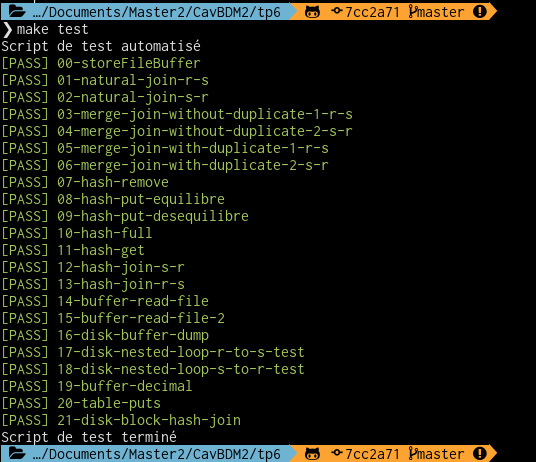
\includegraphics[width=0.8\textwidth]{test.png}

\end{document}
